This section discusses the sources of the estimated gender differences. A major determinant is the choice of the alternative child care arrangements.
Estimated treatment effects are very similar across genders comparing treatment to staying at home full time. Males benefit much more from treatment relative to low quality childcare compared to their benefits from treatment relative to staying at home. This result is consistent with previous research that shows (i) substantial gender differences resulting from attending low quality childcare \citep{Kottelenberg-Lehrer_2014_Gender-Effects,Baker_Gruber_Milligan_2015_Noncog_Defects}; and (ii) that females are less sensitive to more stressful, low quality environments (see, e.g., \citealp{golding2016psychology,Autor-etal_2015_Family-Disadvantage}).

Table~\ref{tab:proportion-table-ranksign} shows the proportion of outcomes by category for which the male outcomes exceed those of females. In Appendix~\ref{appendix:genderdifferences}, we further divide the control group into the alternatives used and both the treatment and control groups by father present, a potentially important moderator. Recall, we condition on baseline variables to control for selection into childcare for controls.\footnote{See Appendix~\ref{appendix:amethodology} \textbf{[JJH: Appendix E! On page 14 we say E!]} for a sensitivity study using other methods. They produce the same estimates, but are less precisely estimated.} Figure~\ref{fig:proportion-altpre} shows the proportions partitioned by alternative childcare setting. The males who stay at home do better than the females in cognitive and parenting measures, employment, and across all outcomes. Unlike the males who attend lower quality alternative childcare, the males who stay at home have similar crime outcomes as the females. Given the important negative effects of male criminal activity, this finding highlights the magnitude of harm caused by low-quality alternative preschools for the males.

\begin{figure}[H]
\centering
\caption{Proportion of Outcomes Males $>$ Females, by Outcome Category, Partitioning by Alternative Childcare Setting}
\label{fig:proportion-altpre}
	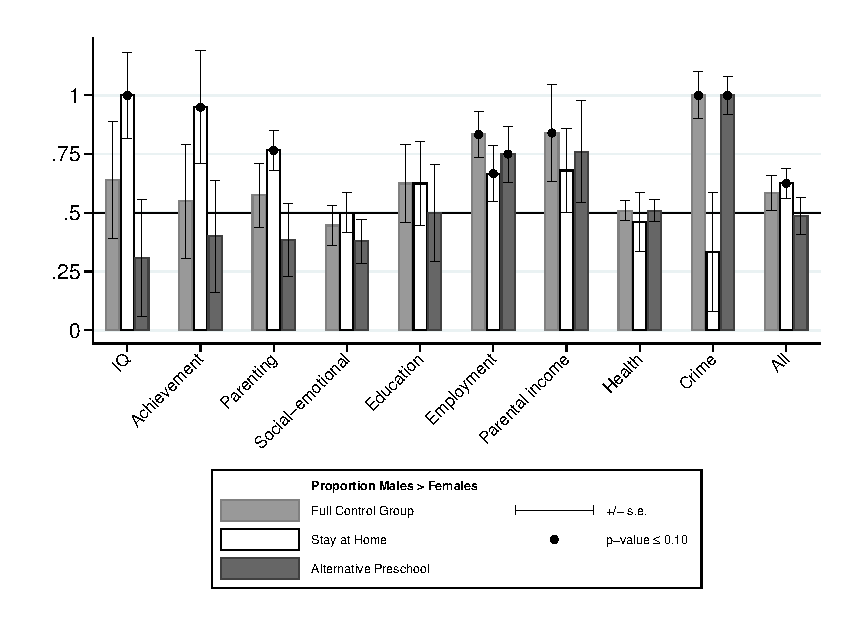
\includegraphics[width=\textwidth]{output/gendergaps-control-moderated-altpre}
\footnotesize \justify
Note: These plots show the proportion of outcomes, by outcome category, for which the males' mean is larger than the females' mean. The standard errors and the $p$-values are computed using 1,000 bootstraps. The $p$-values are one-sided and test the null hypothesis that the proportion of outcomes is greater than $\frac{1}{2}$ The crime outcomes are all coded so that a higher value indicates more criminal activity. All other outcome categories have higher values corresponding to socially desirable outcomes.
\end{figure}

In Appendix~\ref{appendix:genderdifferences}, we report estimates by whether or not the father is present (Figure~\ref{fig:proportion-fhome}). Few clear-cut patterns emerge. Father's presence interacted with treatment favors males for IQ, parenting, and health measures. Males in the control group do better when the father is absent in education and employment. \textbf{[JJH: The results for fathers present and absent are very difficult to interpret.]}

\textbf{[JJH: Writing unclear. Is high good? Clarify.]}

Another measure of home environment is maternal locus of control which is measured when the subjects were 1.5 years old.\footnote{We define internal locus of control as scoring below the sample mean and an external locus of control as scoring at or above the sample mean. See \citet{Rotter_1966_PMGaA}.} A high level of internal locus of control indicates feeling in control of future outcomes, including those related to child rearing. \textbf{[JJH: Internal + external = constant?]} In contrast, a high score on external locus of control indicates feeling that outside forces determine future outcomes (e.g. luck). Figure~\ref{fig:proportion-mlocus} shows empirical results from conditioning on this variable. In the control group, a higher maternal internal locus of control promotes better outcomes for males across all outcome categories except health. Another way to state this is that males are more negatively affected if their mothers have a lower external locus of control than are females. This is consistent with the analyses of \citet{Schore_2017_IMHJ} and \citet{golding2016psychology}. Although locus of control does not necessarily measure depression, this finding corresponds with \citet{Beeghly-etal_2017_IMHJ}, who find that increased maternal depression lead to worse outcomes for young males relative to females.

\begin{figure}[!htbp]
\centering
\caption{Proportion of Outcomes Males $>$ Females, by Outcome Category, Dividing by Maternal Locus of Control}
\label{fig:proportion-mlocus}
\begin{subfigure}[h]{0.7\textwidth}
	\centering
	\caption{Control Group}
	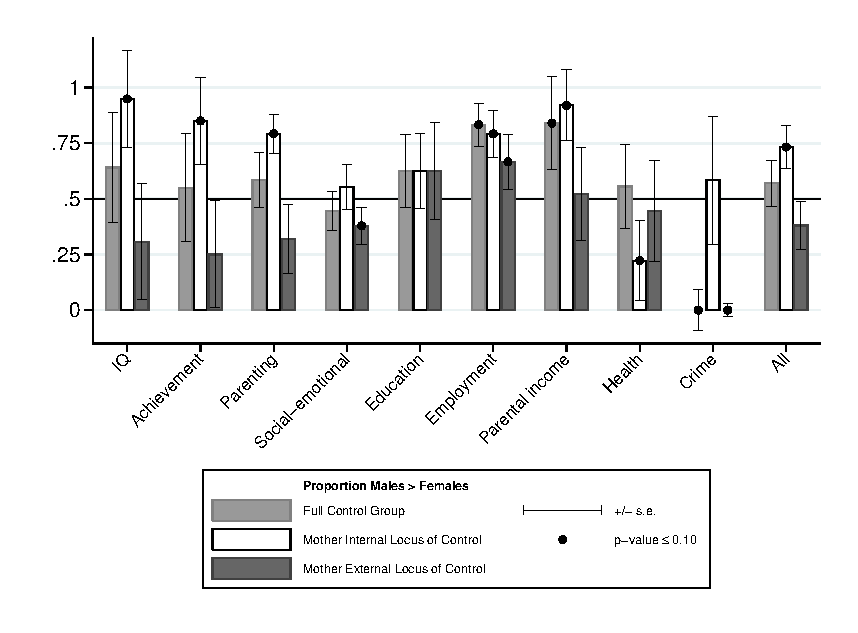
\includegraphics[width=\textwidth]{output/gendergaps-control-moderated-mlocus}
	\end{subfigure}
	
\begin{subfigure}[h]{0.7\textwidth}
	\centering
	\caption{Treatment Group}
	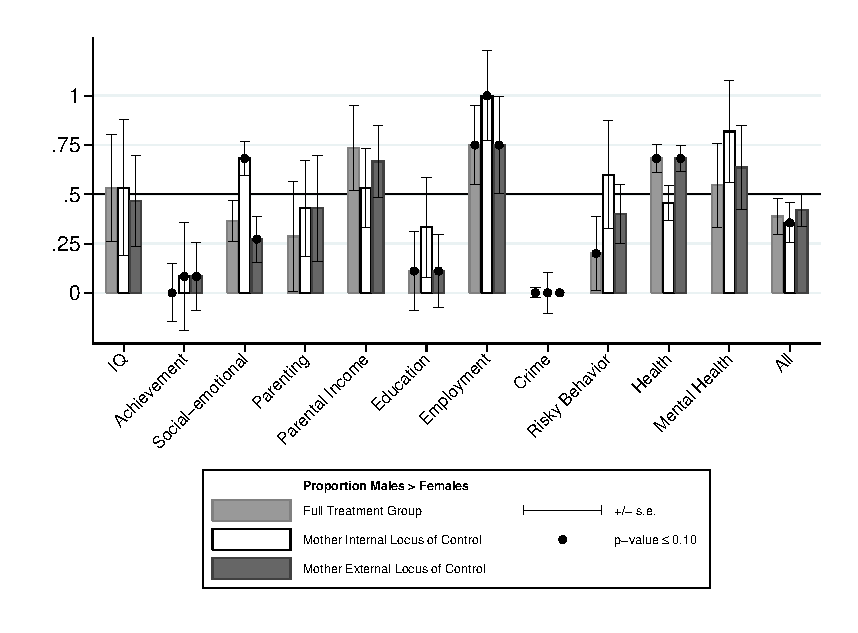
\includegraphics[width=\textwidth]{output/gendergaps-treatment-moderated-mlocus}
	\end{subfigure}
\footnotesize \justify
Note: These plots show the proportion of outcomes, by outcome category, for which the males' mean is larger than the females' mean. The standard errors and the $p$-values are computed using 1,000 bootstraps. The $p$-values are one-sided and test the null hypothesis that the proportion of outcomes is greater than $\frac{1}{2}$ The crime outcomes are all coded so that a higher value indicates more criminal activity. All other outcome categories have higher values corresponding to socially desirable outcomes.
\end{figure}

Maternal locus of control moderates the treatment outcomes differently. Regardless of the level of maternal locus of control, males do not have better outcomes than their female counterparts. The exception is for health outcomes for this outcome of boys with mothers with external loci of control outperform those with mothers with internal loci of control. Treatment compensates for this form of disadvantage. Aggregating across outcomes, male outcomes are not much affected by the mother's locus of control if they attend ABC/CARE, while if they are in the control group, it does. This suggests an important compensating role of enriched early childhood programs.



